%%
%% Copyright 2007, 2008, 2009 Elsevier Ltd
%%
%% This file is part of the 'Elsarticle Bundle'.
%% ---------------------------------------------
%%
%% It may be distributed under the conditions of the LaTeX Project Public
%% License, either version 1.2 of this license or (at your option) any
%% later version.  The latest version of this license is in
%%    http://www.latex-project.org/lppl.txt
%% and version 1.2 or later is part of all distributions of LaTeX
%% version 1999/12/01 or later.
%%
%% The list of all files belonging to the 'Elsarticle Bundle' is
%% given in the file `manifest.txt'.
%%

%% Template article for Elsevier's document class `elsarticle'
%% with numbered style bibliographic references
%% SP 2008/03/01
%%
%%
%%
%% $Id: elsarticle-template-num.tex 4 2009-10-24 08:22:58Z rishi $
%%
%%
%\documentclass[preprint,12pt,3p]{elsarticle}

%% Use the option review to obtain double line spacing
\documentclass[preprint,12pt]{elsarticle}

%% Use the options 1p,twocolumn; 3p; 3p,twocolumn; 5p; or 5p,twocolumn
%% for a journal layout:
%% \documentclass[final,1p,times]{elsarticle}
%% \documentclass[final,1p,times,twocolumn]{elsarticle}
%% \documentclass[final,3p,times]{elsarticle}
%% \documentclass[final,3p,times,twocolumn]{elsarticle}
%% \documentclass[final,5p,times]{elsarticle}
%% \documentclass[final,5p,times,twocolumn]{elsarticle}

%% if you use PostScript figures in your article
%% use the graphics package for simple commands
%% \usepackage{graphics}
%% or use the graphicx package for more complicated commands
%% \usepackage{graphicx}
%% or use the epsfig package if you prefer to use the old commands
%% \usepackage{epsfig}

%% The amssymb package provides various useful mathematical symbols
\usepackage{amssymb}
%% The amsthm package provides extended theorem environments
%% \usepackage{amsthm}

%% The lineno packages adds line numbers. Start line numbering with
%% \begin{linenumbers}, end it with \end{linenumbers}. Or switch it on
%% for the whole article with \linenumbers after \end{frontmatter}.
\usepackage{lineno}
\usepackage[superscript]{cite}

%% natbib.sty is loaded by default. However, natbib options can be
%% provided with \biboptions{...} command. Following options are
%% valid:

%%   round  -  round parentheses are used (default)
%%   square -  square brackets are used   [option]
%%   curly  -  curly braces are used      {option}
%%   angle  -  angle brackets are used    <option>
%%   semicolon  -  multiple citations separated by semi-colon
%%   colon  - same as semicolon, an earlier confusion
%%   comma  -  separated by comma
%%   numbers-  selects numerical citations
%%   super  -  numerical citations as superscripts
%%   sort   -  sorts multiple citations according to order in ref. list
%%   sort&compress   -  like sort, but also compresses numerical citations
%%   compress - compresses without sorting
%%
%% \biboptions{comma,round}

% \biboptions{}

\usepackage{graphicx}
\usepackage[space]{grffile}
\usepackage{latexsym}
\usepackage{textcomp}
\usepackage{longtable}
\usepackage{tabulary}
\usepackage{booktabs,array,multirow}
\usepackage{amsfonts,amsmath,amssymb}
\providecommand\citet{\cite}
\providecommand\citep{\cite}
\providecommand\citealt{\cite}
\usepackage{url}
\usepackage{hyperref}
\hypersetup{colorlinks=false,pdfborder={0 0 0}}
\usepackage{etoolbox}
\makeatletter
\patchcmd\@combinedblfloats{\box\@outputbox}{\unvbox\@outputbox}{}{%
  \errmessage{\noexpand\@combinedblfloats could not be patched}%
}%
\makeatother
% You can conditionalize code for latexml or normal latex using this.
\newif\iflatexml\latexmlfalse
\providecommand{\tightlist}{\setlength{\itemsep}{0pt}\setlength{\parskip}{0pt}}%

\AtBeginDocument{\DeclareGraphicsExtensions{.pdf,.PDF,.eps,.EPS,.png,.PNG,.tif,.TIF,.jpg,.JPG,.jpeg,.JPEG}}

\usepackage[utf8x]{inputenc}
\usepackage[T1]{fontenc}
\usepackage[greek,english]{babel}

% Use this header.tex file for:
% 1. frontmatter/preamble LaTeX definitions
%  - Example: \usepackage{xspace}
% 2. global macros available in all document blocks
%  - Example: \def\example{This is an example macro.}
%
% You should ONLY add such definitions in this header.tex space,
%  and treat the main article content as the body/mainmatter of your document
% Preamble-only macros such as \documentclass and \usepackage are
% NOT allowed in the main document, and definitions will be local to the current block.
\newcommand{\energy}{\mathcal{E}}

\makeatletter
% Authorea add-on: ensure doi defined
\providecommand{\doi}[1]{%
  \begingroup
    \let\bibinfo\@secondoftwo
    \urlstyle{rm}%
    \href{http://dx.doi.org/#1}{%
      doi:\discretionary{}{}{}%
      \nolinkurl{#1}%
    }%
  \endgroup
}

\def\ps@pprintTitle{%
 \let\@oddhead\@empty
 \let\@evenhead\@empty
 \let\@oddfoot\@empty%
 \let\@evenfoot\@oddfoot}

\makeatother

\journal{Elsevier Journal}

\begin{document}
\begin{frontmatter}

%% Title, authors and addresses

%% use the tnoteref command within \title for footnotes;
%% use the tnotetext command for the associated footnote;
%% use the fnref command within \author or \address for footnotes;
%% use the fntext command for the associated footnote;
%% use the corref command within \author for corresponding author footnotes;
%% use the cortext command for the associated footnote;
%% use the ead command for the email address,
%% and the form \ead[url] for the home page:
%%
%% \title{Title\tnoteref{label1}}
%% \tnotetext[label1]{}
%% \author{Name\corref{cor1}\fnref{label2}}
%% \ead{email address}
%% \ead[url]{home page}
%% \fntext[label2]{}
%% \cortext[cor1]{}
%% \address{Address\fnref{label3}}
%% \fntext[label3]{}

\title{Quantitative lung microstructure mapping with X-ray dark-field grating
interferometry on a laboratory source}



\author[add1,add2]{Matteo Abis}%
\author[add2]{Goran Lovrić}%
\author[add3]{Johannes Schittny}%
\author[add1,add2]{Marco Stampanoni}%
\author[add4]{Tiziana Cremona}%
\author[add3]{Charaf Benarafa}%
\address[add1]{ETH Zurich}%
\address[add2]{Paul Scherrer Institute}%
\address[add3]{University of Bern}%
\address[add4]{Harvard School of Public Health}%

\selectlanguage{english}
\begin{abstract}
A wide range of pulmonary diseases affect the lungs microstructure, i.e.
the alveolar epithelium, where diffusion-driven gas exchange takes
place.~ Thereby, early and definite diagnosis is not only important to
prevent treatment delays, but also to counteract acute exacerbation and
initiate treatment before reaching an irreversible state. In a number of
works, dark-field grating interferometry has been identified as the most
promising technique in the screening of disease-induced changes to the
lungs microstucture, most notably in the early diagnosis of pulmonary
emphysema. Particularly the dependency of the small-angle scattering
(dark-field)~signal on the mean alveolar size has the potential to
improve diagnosis. On the other hand, it has also been shown that the
dark-field signal can be strongly biased and system-dependent when
acquired on a conventional X-ray tube. In the present work, we present a
full model-driven framework for quantitatively mapping the lungs
microstructure to the dark-field image. Starting from first principles,
our quantitative model for dark-field radiography on a laboratory source
is verified~ with high-resolution (sub-micron scale) tomographic volumes
of the same samples. We show that our model is capable of establishing a
direct correlation between microstructure and the macroscopic X-ray
radiographic image. This provides a deeper understanding of dark-field
imaging that can be beneficial for the design of an interferometer as a
specific diagnostic tool, as well as for similar analyses in different
fields of foam dynamics and material sciences. (Goran: last sentence I
would still adapt depending on what really the conclusion is: ideally
already suggest an idealistic interferometer and/or imaging
technique\ldots{})%
\end{abstract}%



%\begin{keyword}
%% keywords here, in the form: keyword \sep keyword

%% MSC codes here, in the form: \MSC code \sep code
%% or \MSC[2008] code \sep code (2000 is the default)

%\end{keyword}

\end{frontmatter}
\linenumbers



\section*{Introduction}\label{sec:introduction}
First paragraph (Goran can write) BACKGROUND ABOUT LUNG
The problems with lung diseases are multifaceted. Lung diseases are diagnosed at an already progressed state at which they are not reversible. On the other hand, many conditions like asthma, chronic obstructive pulmonary disease (COPD) and bronchiectasis exhibit very heterogeneous conditions Hence, the key challenges still remain: early diagnosis, efficient therapy (once a disease is diagnosed) and prediction in both follow-up and outcome [refs]. Typical diagonstic tool is chest-Xray byt state of the art is HRCT...Final diagnosis via collaboration with pathology...

X-ray grating interferometry has been developed over the course of the last
  fifteen years on both synchrotron and laboratory
sources~\cite{David_2002,1347-4065-42-7B-L866,Weitkamp_2005,1347-4065-45-6R-5254,Pfeiffer2006}. Interferometric
imaging allows simultaneous access to three independent images: the
conventional absorption image, a differential phase signal and a dark-field
signal, also known as visibility contrast. This last signal has been
reported by multiple sources as being quantitatively linked to the presence
of unresolved structures in the sample, much smaller than the pixel size of
the detector, and typically of the order of the
micrometer~\cite{Pfeiffer2008,Lynch:11,Yashiro:10}.
Various clinically relevant
applications~\cite{Wen_2009,Thilo2013} have been
proposed, including lung microstructural analyses~\cite{Schleede17880,Meinel_2014,Meinel_2013,Yaroshenko_2013,Modregger2016}.

In particular, emphysema is a pathological condition of the lung
resulting in structural changes in the alveoli, that is at the smallest
hierarchical level in the tissue. These changes are caused by the
destruction of interalveolar septa, with larger air spaces progressively
replacing the fine architecture of the lung parenchyma~\cite{Sharafkhaneh_2008}. These larger spaces
have a less favorable surface-to-volume ratio, thus lowering the efficiency
of respiratory exchanges. Previous studies on murine lungs established that the increased sensitivity of
the dark-field signal of an X-ray grating interferometer to micrometer-sized
features can distinguish between emphysematous from healthy samples and
provide a mapping of the parenchyma showing the localization of the
structural damage. The strength of the dark-field signal in grating interferometry is
given by the small-angle scattering of X-rays by structures smaller than the
spatial resolution of the imaging system, after taking into account the effects of beam hardening for polychromatic sources~\cite{Koenig2016}. The lung is therefore an ideal
application for this technique, since the alveoli are much
smaller than the spatial resolution available for chest radiography.

In this work we present a quantitative model of the dark-field signal
generated by lung tissue in an X-ray grating interferometer on a laboratory
source. High-resolution tomographic data resolving the features down to single
alveoli is analyzed with established post-processing techniques to extract a
ground truth on the sizes of the structures composing the lung tissue. The
lung is then modeled as a suspension of spheres of different sizes in a
homogeneous medium~\cite{Kitchen2004, Carnibella2012a, Leong2014}, in the hypothesis that the signals generated by spheres
of different sizes and by X-rays of different energies sum up incoherently.
Finally, an X-ray interferometric radiography on a laboratory source is
recorded, to allow a direct comparison between the expected dark-field
signal calculated according to this model and the experimental values.

\section*{Results}\label{sec:model}
\subsection*{Extension to a polychromatic model}
Previous works~\cite{Lynch:11,Gkoumas2016} have demonstrated quantitative estimation of
the dark-field signal for a monochromatic source and monodisperse solutions
of micrometer-sized spheres. In particular, the coefficient $\mu_B$, for a
beam of wavelength $\lambda$ is:

\begin{equation}
\mu_B = \frac{3\pi}{\lambda^2}f |\Delta n|^2 d
    \begin{cases}
    D' & \text{if } D' \leqslant 1\\
    \begin{aligned}
    D' - \sqrt{D'^2 - 1}\\
    (1 + D'^{-2}/2) \\
    + (D'^{-1} + D'^{-3} / 4) \\
    \log\left(\frac{D' + \sqrt{D'^2 - 1}}{D' - \sqrt{D'^2 - 1}}\right)
    \end{aligned} & \text{otherwise.}
    \end{cases}
    \label{eqn:lynch}
\end{equation}

The autocorrelation length is $d = L\lambda / p$ with $L$ the sample to
detector distance, $p$ and the period of $G_2$. $D'$ is a normalized
particle diameter equal to $D/d$, where $D$ is the particle diameter. $f$ is
the fraction of volume occupied by the scattering material and $n = 1 -
\delta - i\beta$ is the complex refractive index.

We rewrite this formula more concisely as

\begin{equation}
    \mu_B(\energy) = C |\Delta n(\energy)|^2 \energy u(\energy),
    \label{eqn:lynchshort}
\end{equation}
where $\energy$ is the energy of the beam, $C = 3 fL / 4p$ is a constant
depending only on the setup geometry and the volume fraction $f$ occupied by
the spheres and $\energy$ is the energy of the beam.


In the case of a polychromatic source, we tested a model where different
energies interact with the sample independently of each other, thus allowing
an incoherent sum of the dark-field signals over the spectral weights
$s(\energy)$:

\begin{equation}
    R = C \frac{\sum_\energy s(\energy)|\Delta n(\energy)|^2 \energy u(\energy)}{\sum_\energy s(\energy) \energy \beta}.
    \label{eqn:lynchpolychromatic}
\end{equation}

This formula was first tested on monodisperse solution of silicon dioxide
spheres with sizes ranging from 0.166 \selectlanguage{greek}μ\selectlanguage{english}m to 7.760 \selectlanguage{greek}μ\selectlanguage{english}m, with a volume fraction of 20\%
in glycerine. This model yields a good agreement between the continuous line
and the experimental data representing radiographies of the silicon dioxide
sphere samples recorded on the laboratory source interferometer.\selectlanguage{english}
\begin{figure}[h!]
\begin{center}
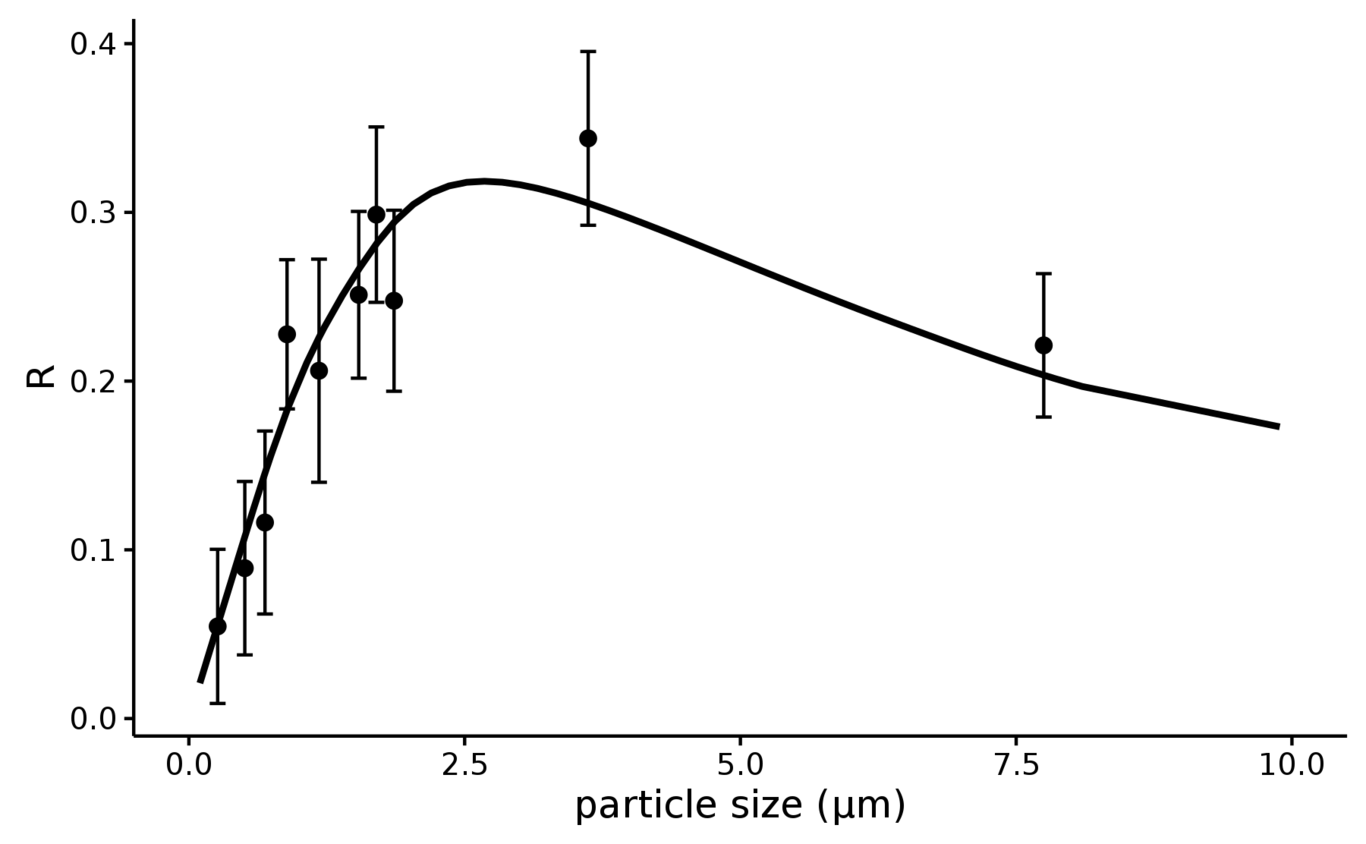
\includegraphics[width=0.70\columnwidth]{figures/summary/summary}
\caption{{Silicon dioxide monodisperse microspheres in a 20\% solution of
glicerine. as a function of sphere diameter. The continuous line is the
function in eq. {\ref{eqn:lynchpolychromatic}}.
{\label{725462}}%
}}
\end{center}
\end{figure}


A model of the sample is required to calculate the spectral weights
$s(\energy)$ in order to avoid beam hardening artefacts. The source spectrum is
simulated with the SpekCalc~\cite{spekcalc} software, then attenuated
according to NIST absorption tables~\cite{Hubbell_1995} for the sample in the beam path and the
efficiency of the detector.

In this work, we propose to model the lung sample as a solution of
polydisperse spherical air bubbles embedded in tissue. The distribution of
the sphere diameters is extracted from the microtomographic data, together
with the fraction of the volume occupied by the tissue. The density of the
tissue is also estimated from tomographic projections: the composition is
taken from the ICRU-44 lung tissue tables~\cite{White_1989}, while the density is increased to
1.6 g/cm$^3$ as to match the absorption values recorded on the tomographic
projections. This results from the drying procedure for the fixation of
the samples, leaving a denser material than in \emph{in vivo} conditions.

The coefficient $\mu_B$ can then be expressed as a double summation over the spectrum
$s(\energy)$ and over the distribution of sphere diameters $\rho(d)$:

\begin{equation}
    \mu_{B,\text{total}} = \sum_{d}\sum_{\energy} \mu_B(r, E; n, f)\rho(d)s(\energy)
    \label{eqn:totalsum}.
\end{equation}


\subsection*{Tube and synchrotron analysis of lung samples}
The section of the radiographic image of each lung sample is manually
matched to the local tomography, as identified during the alignment of the
tomographic scan. The average and standard deviation of the $R$ values are
calculated and plotted in fig.~\ref{206272} (black dots and errorbars). The expected
values according to eq.~\ref{eqn:totalsum} are calculated with the inputs from the
microtomographic datasets, as described in section~\ref{sec:tomoprocessing}, and are plotted on
fig.~\ref{206272} with red dots for each sample.\selectlanguage{english}
\begin{figure}[h!]
\begin{center}
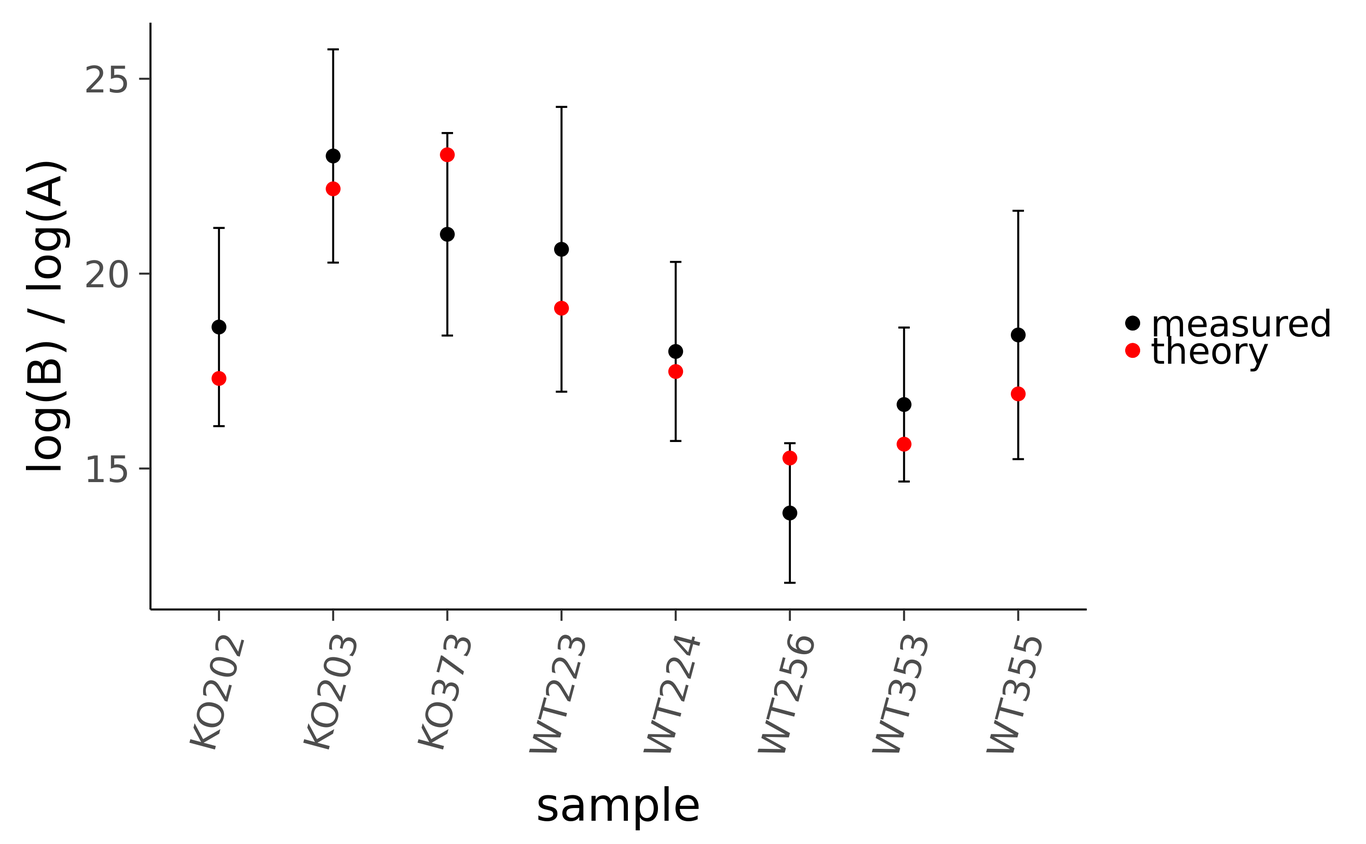
\includegraphics[width=0.70\columnwidth]{figures/samples/samples}
\caption{{Value log(B)/log(A) for each lung in the laboratory setup radiography
(measured, black dots with errorbars) compared to the expected value
modelled from microtomographic inputs (theory).
{\label{206272}}%
}}
\end{center}
\end{figure}


The measured data agreed with the
theory for all samples, and the $\chi^2$ statistic can be calculated

\begin{equation}
    \chi^2 = \sum_{i=1}^8 \dfrac{(R_{\text{obs}} -
    R_{\text{th}})^2}{\mathop{\mathrm{Var}}(R_{\text{obs}})} = 2.31.
    \label{eqn:chisq}
\end{equation}

With 7 degrees of freedom, this results in a right-tail probability of 0.94 that the 
observations are consistent with the model, thus validating the quantitative estimation of
dark-field values for a lung model as a collection of incoherently
superimposed microscopic spheres.

\section*{Discussion}
Possible sources of inaccuracy of our model include a significantly
different distribution of shapes in the lung parenchyma, or additional
effects of beam hardening which are known to influence the dark-field
signal. In order to consider the effects of possible shape asymmetries, a
single mouse lung sample was scanned at the X02DA TOMCAT beamline with the
setup described in Kagias et al.~\cite{PhysRevLett.116.093902}. This
technique is similar to Talbot interferometry, but it is able to detect
scattering from unresolved microscopic structures under different angles in
a single shot by
creating an array of circular interference patterns. The intensity of the
dark-field signals for different angles can then be recovered for each
pixel, and an asymmetry value defined as the amplitude of this periodic
signal divided by the average can be calculated for each pixel. This allows
us to exclude the possibility that there are significant inhomogeneities in
the dark-field response of the lung structures under different angles, which
would directly invalidate the model of a superposition of spheres. This
amounts to quantifying the departure from a spherical model towards
ellipsoids. In our sample this asymmetry is an average of $0.11 \pm 0.04$, indicating a departure from the spherical model of less than 15\%.

Another effect commonly reported in dark-field analyses on wide, polychromatic
sources is the influence of beam hardening on the recorded dark-field
values. In our case, given the high voltage of the source and the small
thickness of the samples (less than 4 mm), the absorption ranges from 4\% to
6\%. The correction to dark-field values provided by is therefore
not applied, as it is reported to be relevant for samples absorbing at least
50\% of the incoming light. The beam hardening effect is considered insofar
it affects the spectral weights of eq.~\ref{eqn:totalsum}, which are calculated
after the sample.

While this setup has a short autocorrelation length of only few micrometers
(figure~\ref{725462}), it would be possible to design a setup that is more
sensitive to the structure sizes found in human lungs, where the alveoli are
larger than
100 \selectlanguage{greek}μ\selectlanguage{english}m~\cite{Ochs_2004}. We can describe a
possible choice of parameters for a Talbot-Lau interferometer for lung
screening. The design energy can be chosen as 60 keV, close to
the mean voltage for a 100 kV setting on a chest
radiography. An intergrating length of 1 m is required to provide
enough room for the patient to comfortably fit the machine,
and a period of 1.2 \selectlanguage{greek}μ\selectlanguage{english}m could be achievable without
excessively stretching the requirements on the fabrication of the optical
elements. This results in an autocorrelation length around
25 \selectlanguage{greek}μ\selectlanguage{english}m, which is large enough to provide contrast according
to the mechanism shown in figure~\ref{725462}, thus providing better contrast than the
current setup.

\section*{Methods}\label{sec:methods}
\subsection*{Sample preparation}
Wild-type 129S6 and SvEv/Tac mice \cite{Dai_2015} were exposed to cigarette smoke for 5 hours per day and 5 days per week for 4 months. This treatment induced a very mild pulmonary emphysema. Controls were exposed to filtered air. Smoke of 3R4F research cigarettes (University of Kentucky, Lexington, KY) was generated as previously described~\cite{Cremona_2013} by a TE10z smoking machine (Teague Enterprises, Woodland, CA) connected to whole-body exposure chambers. The animals were housed in the central animal facility of the University of Bern at a 12/12 hour day/night circle. They received water and food ad libitum. After 4 months of smoking lungs were instilled with 1.5\% paraformaldehyde-1.5\% glutaraldehyde in 0.15 M HEPES pH 7.35 through a tracheal cannula at a constant pressure of 20 cm H2O. After ligating the trachea the lungs were removed and placed in fresh fixative for at least 24 hours to complete fixation~\cite{Cremona_2013}. In order to preserve the delicate structure of the lungs and to prepare them for X-ray imaging, the lungs were washed in PBS and a graduated series of ethanol, followed by critical point drying~\cite{Barr__2016,Kaeslin_2005}.

Handling of the animals before and during the experiments, as well as the experiments themselves, were approved and supervised by the Swiss Agency for Environment, Forests and Landscape and the Veterinary Service of the Canton of Berne. For ethical reasons we were obliged to keep the number of animals as low as possible.

\subsection*{Image acquisition}\label{sec:acquisition}
The high-resolution microtomographic 3D image data were acquired at the X02DA TOMCAT beamline of the Swiss Light Source at the Paul Scherrer Institute (Villigen, Switzerland). The X-ray beam was generated with a 2.9 T superbending magnet from electrons at an energy of 2.4 GeV with synchrotron ring current of 400 mA in top-up mode. A monochromatic X-ray energy of 11 keV was tuned with a double-multilayer monochromator. After penetrating the sample, a 20 \selectlanguage{greek}μ\selectlanguage{english}m thick scintillator (LuAg:Ce) was used to convert the X-rays into visible light and combined with a 10x magnifying visible-light objective to yield an effective pixel size of $0.65 \times 0.65\,$\selectlanguage{greek}μ\selectlanguage{english}m$^2$. A scientific CMOS detector (pco.Edge 5.5) was used with a single-projection exposure time of 100 ms and a total of 1801 tomographic projections. A sample-to-detector distance of approximately 10 mm was employed to yield a good compromise between contrast and spatial resolution and, prior to CT-reconstruction \cite{Marone2012}, phase retrieval was conducted from single defocused images using a transport-of-intensity approximation as originally proposed by Paganin \textit{et al.} \cite{Paganin2002}. Immediately before the tomographic scan, a camera records the position of the lung with respect to the X-ray beam~\ref{603392}. This area is then matched to the radiographs recorded with the Talbot-Lau interferometer.\selectlanguage{english}
\begin{figure}[h!]
\begin{center}
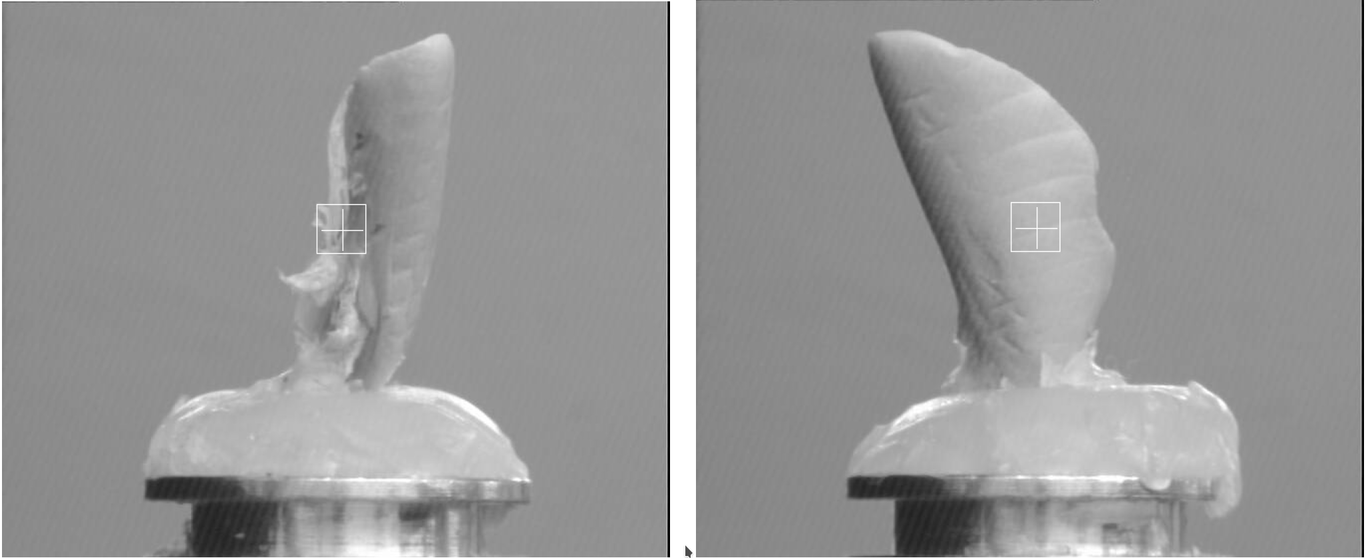
\includegraphics[width=0.70\columnwidth]{figures/Screenshot_20190121_153540/Screenshot_20190121_153540}
\caption{{Alignment positions for the microtomography of the sample labelled
KO202. These are recorded just before each tomographic scan in order to
mark the exact location of~ the scan itself. This is then used to match
the same area from the radiography on the Talbot-Lau interferometer.
{\label{603392}}%
}}
\end{center}
\end{figure}

The radiographies on the laboratory source were taken on a symmetric
Talbot-Lau interferometer (see fig.~\ref{248327}) with a grating pitch of 5.4 \selectlanguage{greek}μ\selectlanguage{english}m and an intergrating
distance of 26 cm, the phase-shift grating provides a phase shift of $\pi$
at 45 keV. The average visibility of the interference pattern without any
sample is 14\%. The source is a Comet MXR-225/26 X-ray tube operated at 100
kV and 6 mA. The source size is 1 mm. The detector is a prototype based on
Santid CdTe by Dectris Ltd. The CdTe 750 \selectlanguage{greek}μ\selectlanguage{english}m sensor provides high quantum
efficiency at high energies (>90\% at 60 keV) with a pixel size of 75 x 75
\selectlanguage{greek}μ\selectlanguage{english}m$^2$. The phase-stepping procedure was performed with 31 phase steps with
1 s exposure per step.\selectlanguage{english}
\begin{figure}[h!]
\begin{center}
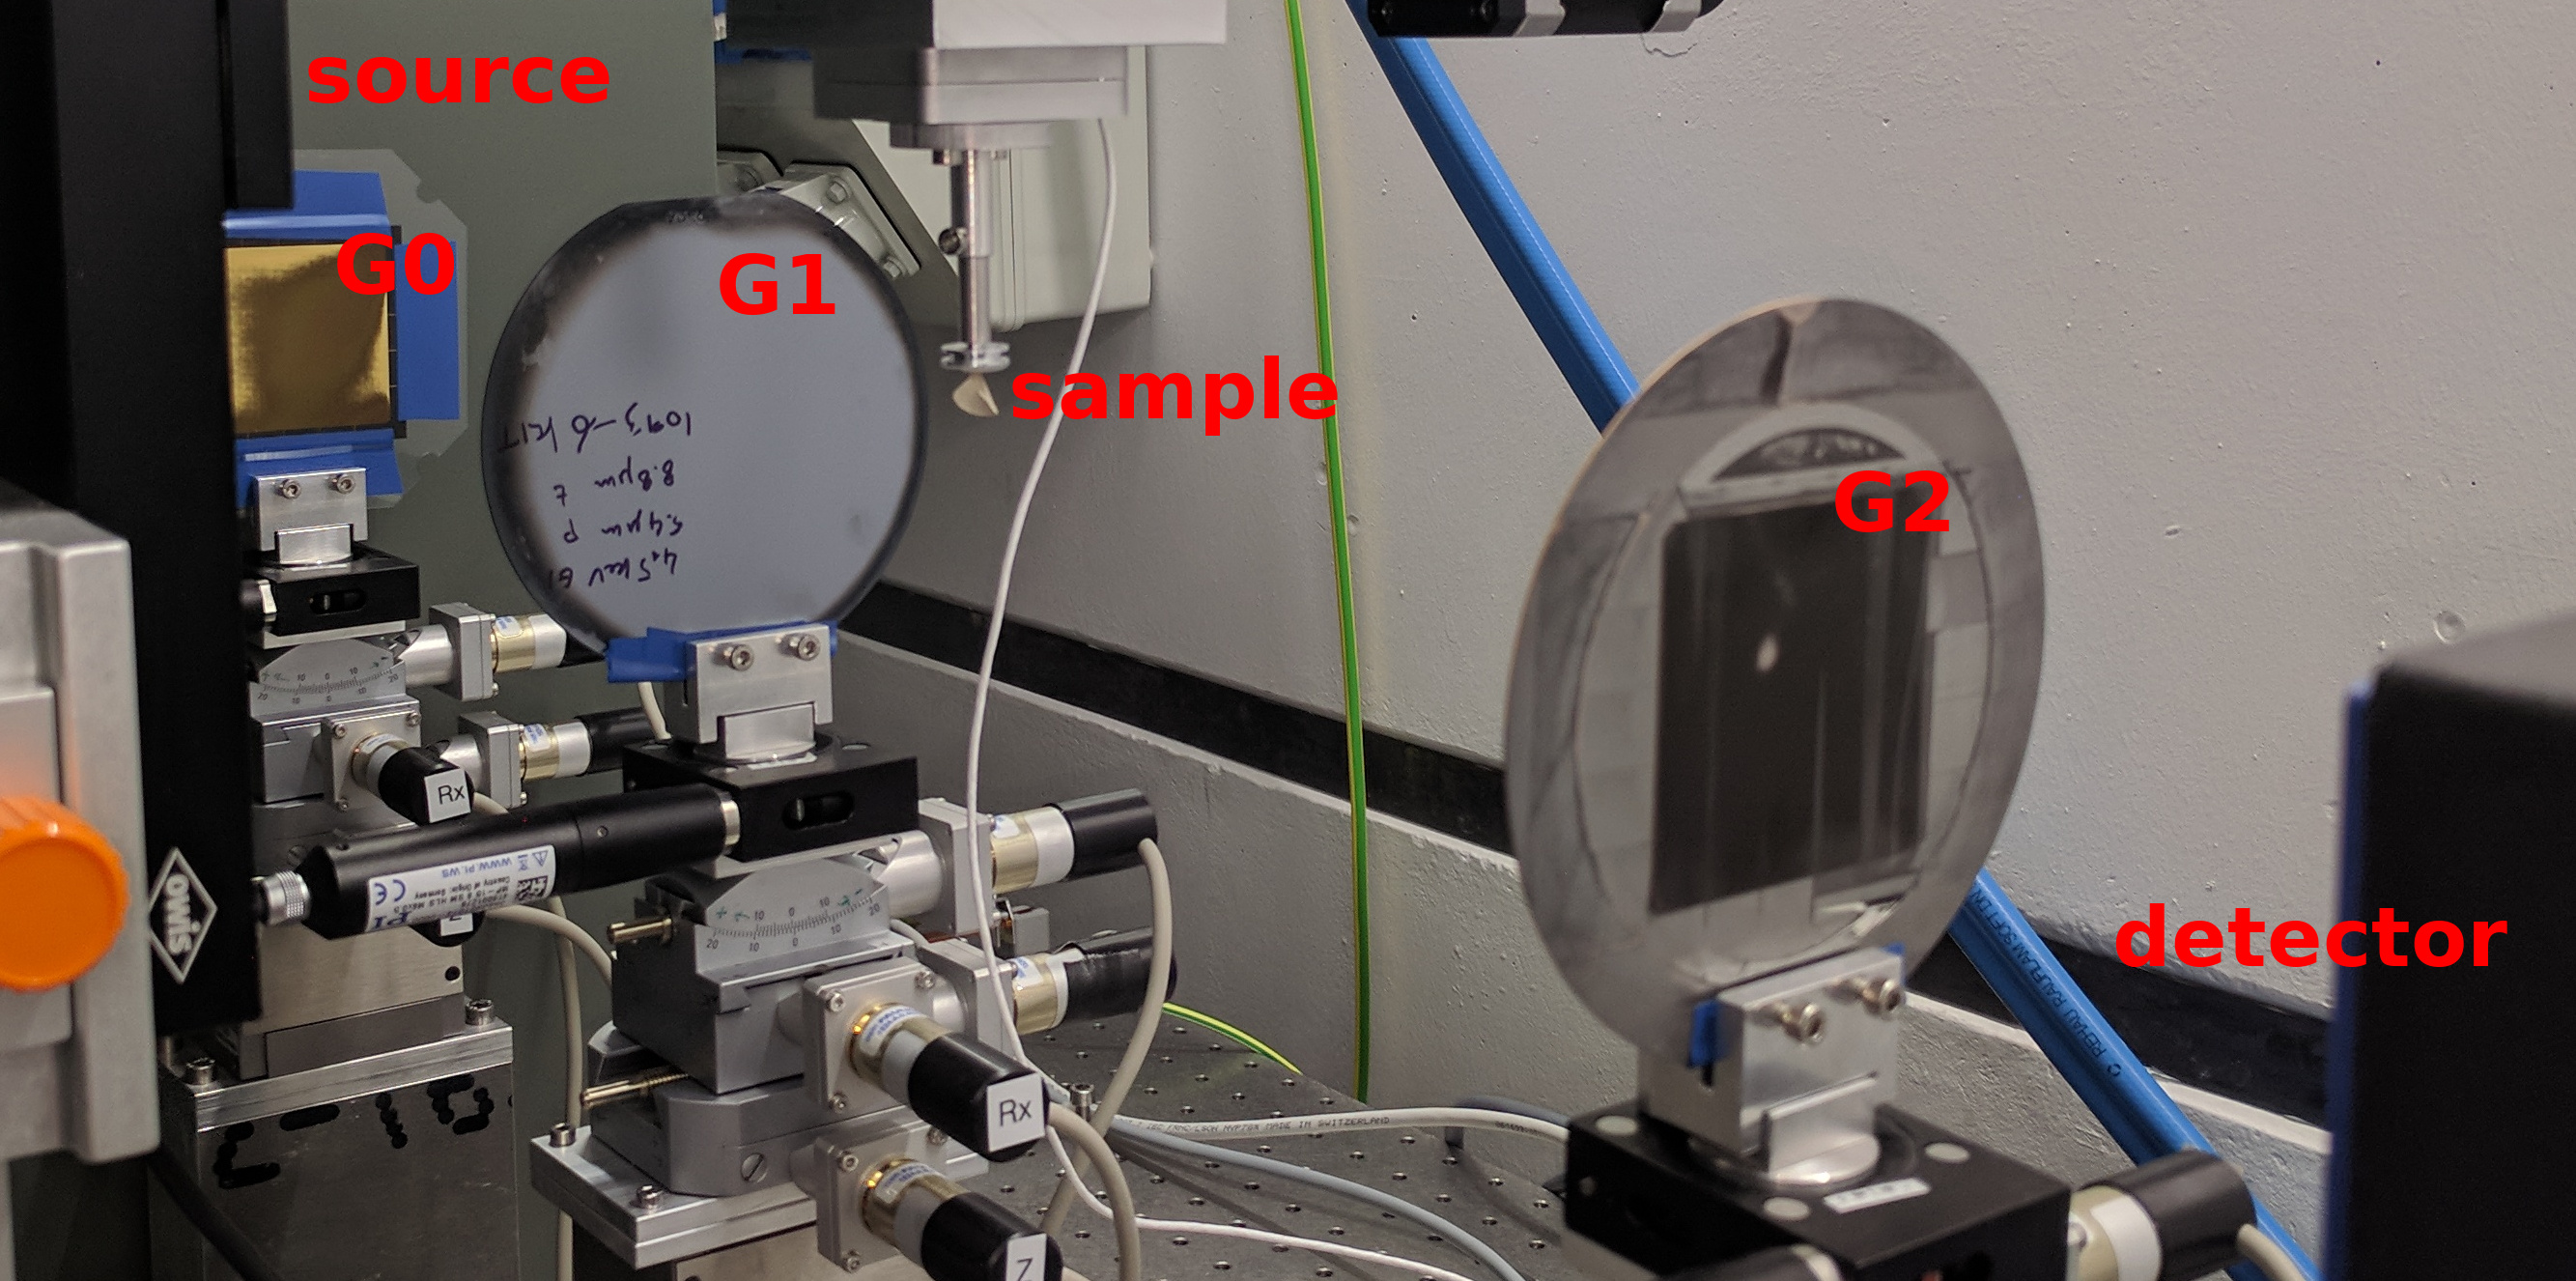
\includegraphics[width=0.70\columnwidth]{figures/lung-setup/lung-setup}
\caption{{RTalbot-Lau interferometer with three gratings G0, G1 and G2, used for
the radiographies on the laboratory source.
{\label{248327}}%
}}
\end{center}
\end{figure}


\subsection*{Processing of the tomographic data}\label{sec:tomoprocessing}
The tomographic sinograms are preprocessed with the Paganin
algorithm~\cite{Paganin_2002a} and
the 3D volume is then reconstructed with the gridrec
algorithm~\cite{Marone_2012}. The volumes, shown in
figure are then thresholded with the Otsu
algorithm~\cite{Otsu_1979}, with independent thresholds for each slice, to
provide a binary labelling for tissue and air. A cycle of
erosion and dilation is applied to remove single pixel artifacts while still
keeping the septa between neighboring alveoli (figure~\ref{591939}).
This preserves the structures in the lung because septa, while possibly
being only one pixel in thickness, are also connected to surrounding tissue.
On the other hand, isolated pixels should be removed as they could affect
the subsequent analysis.\selectlanguage{english}
\begin{figure}[h!]
\begin{center}
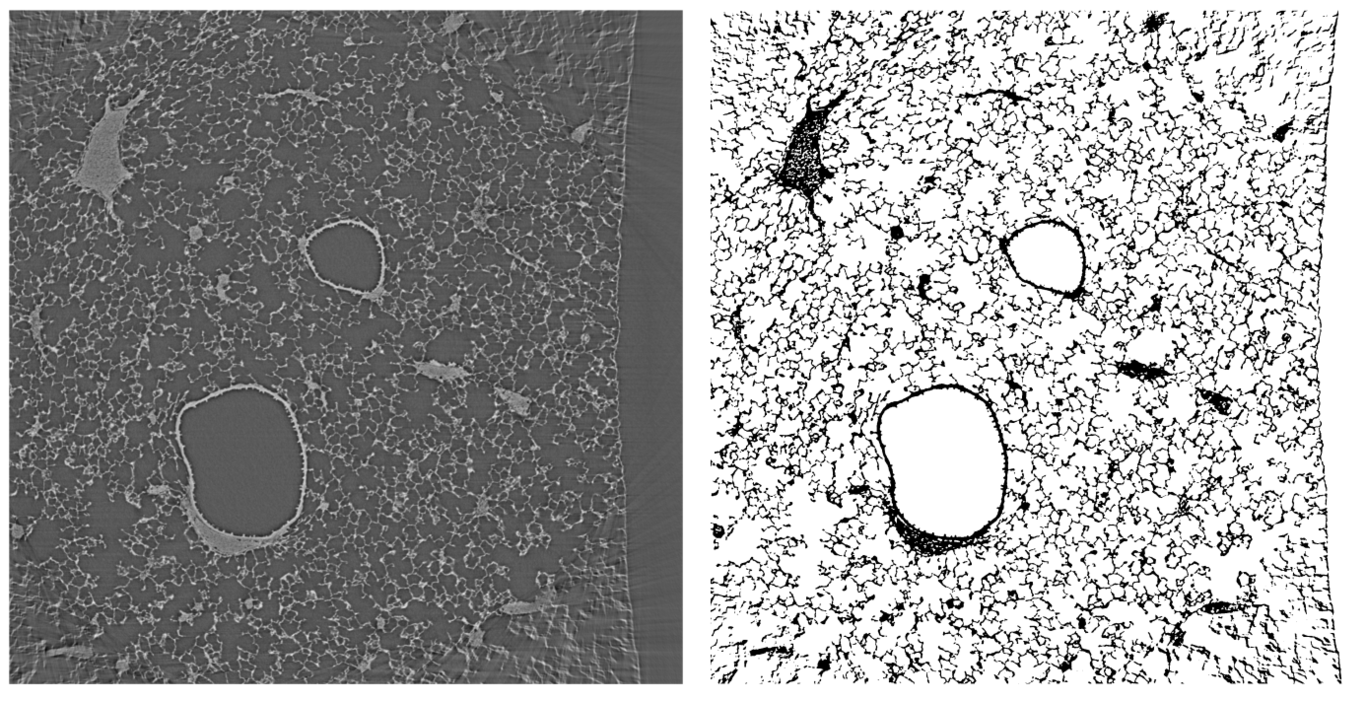
\includegraphics[width=0.70\columnwidth]{figures/reco/reco}
\caption{{Reconstruction (left) and segmentation (right) of a local
microtomography of the sample KO202, performed at the X02DA TOMCAT
beamline.
{\label{591939}}%
}}
\end{center}
\end{figure}


Next, each lung sample is manually stitched from three or four local
tomographies, depending on the sample thickness, and the local air thickness
map is calculated. The local thickness map is an algorithm developed for
bone analysis or foam analysis in material science~\cite{Hildebrand_2003}, that aims
at calculating the maximum diameter of a sphere fitting in each hole in the
sample.
The euclidean distance transform is calculated from the image, yielding the
distance of each point in the airways from the closest
wall.
The points in the transformed dataset are then sorted in descending order in
order to fit the largest possible sphere at each location.
Each of the airways is filled with the largest possible
sphere, resulting in a model where the lung airways are a collection of
spheres embedded in the background of the tissue.\selectlanguage{english}
\begin{figure}[h!]
\begin{center}
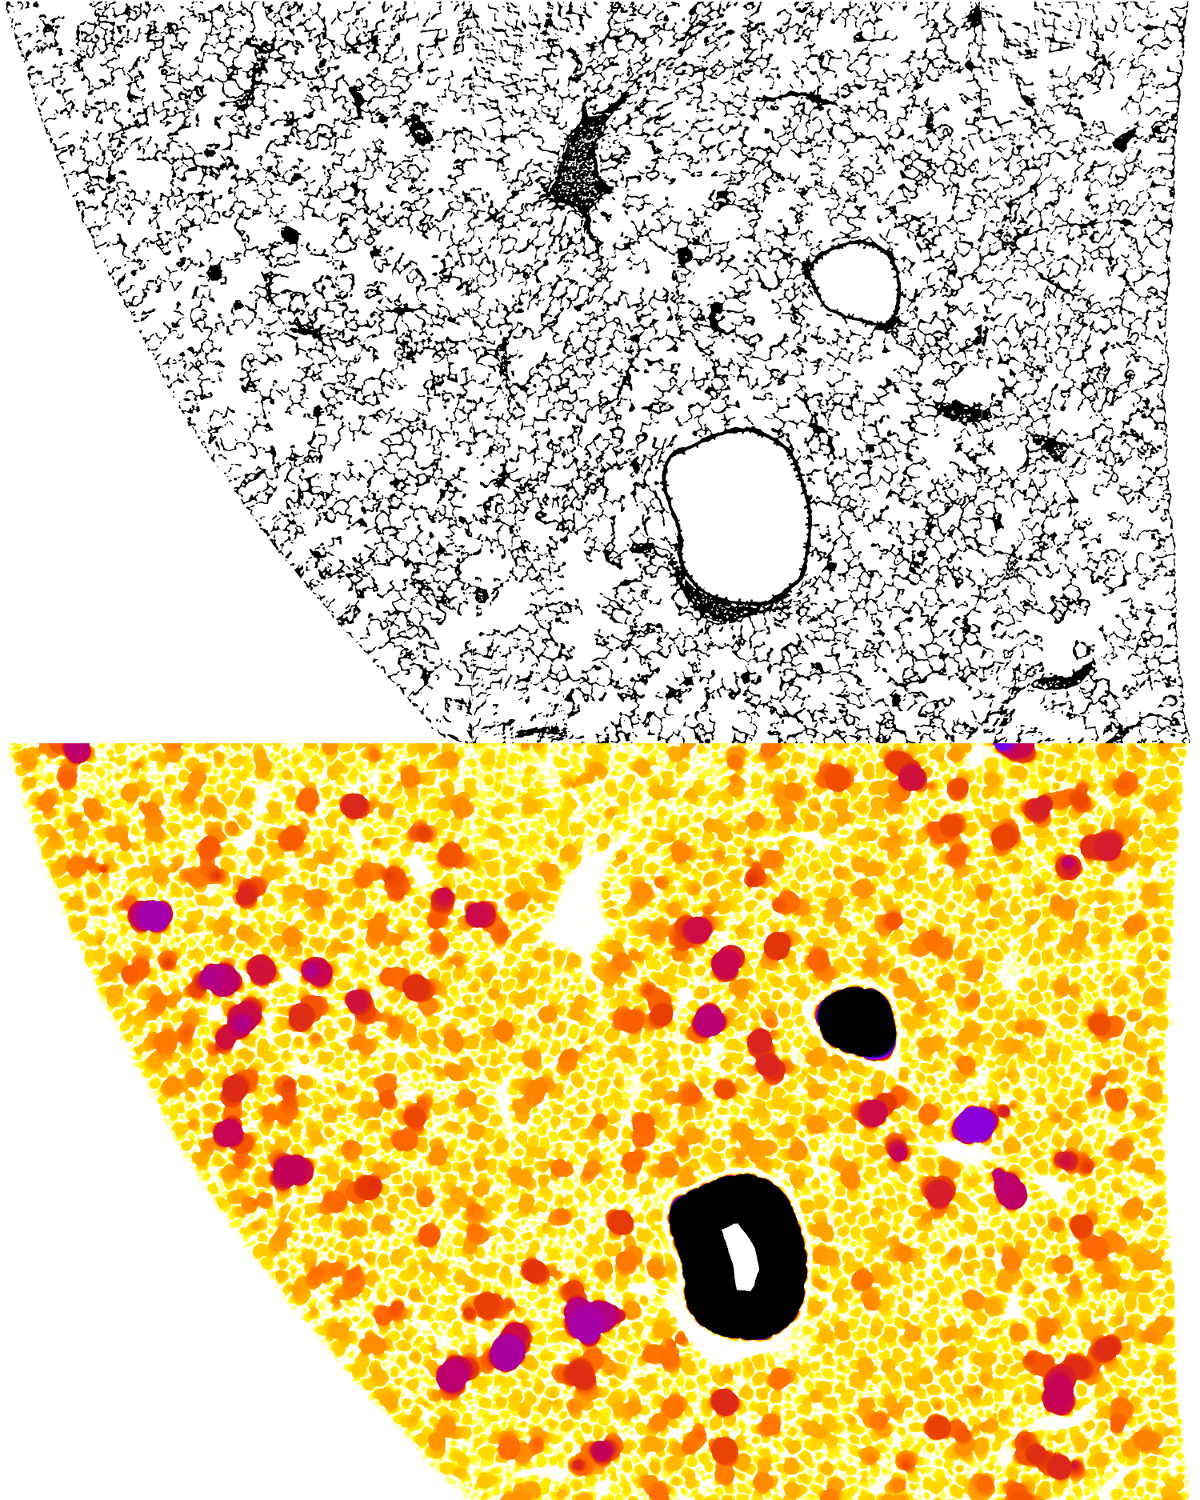
\includegraphics[width=0.70\columnwidth]{figures/thickmap/thickmap}
\caption{{Stitched slice of the mouse lung labelled KO202, measured on the X02DA
TOMCAT beamline (top).~ Thickness map~ where airways are filled with
spheres with the largest diameter that fits between the walls (bottom).
{\label{939269}}%
}}
\end{center}
\end{figure}


To obtain a distribution of sphere sizes (figure~\ref{243343}), kernel density estimation in the R
statistics package \emph{ks}~\cite{Duong_2007} is used in order to avoid possible artifacts
resulting from the arbitrary binning of the histogram of sphere sizes.\selectlanguage{english}
\begin{figure}[h!]
\begin{center}
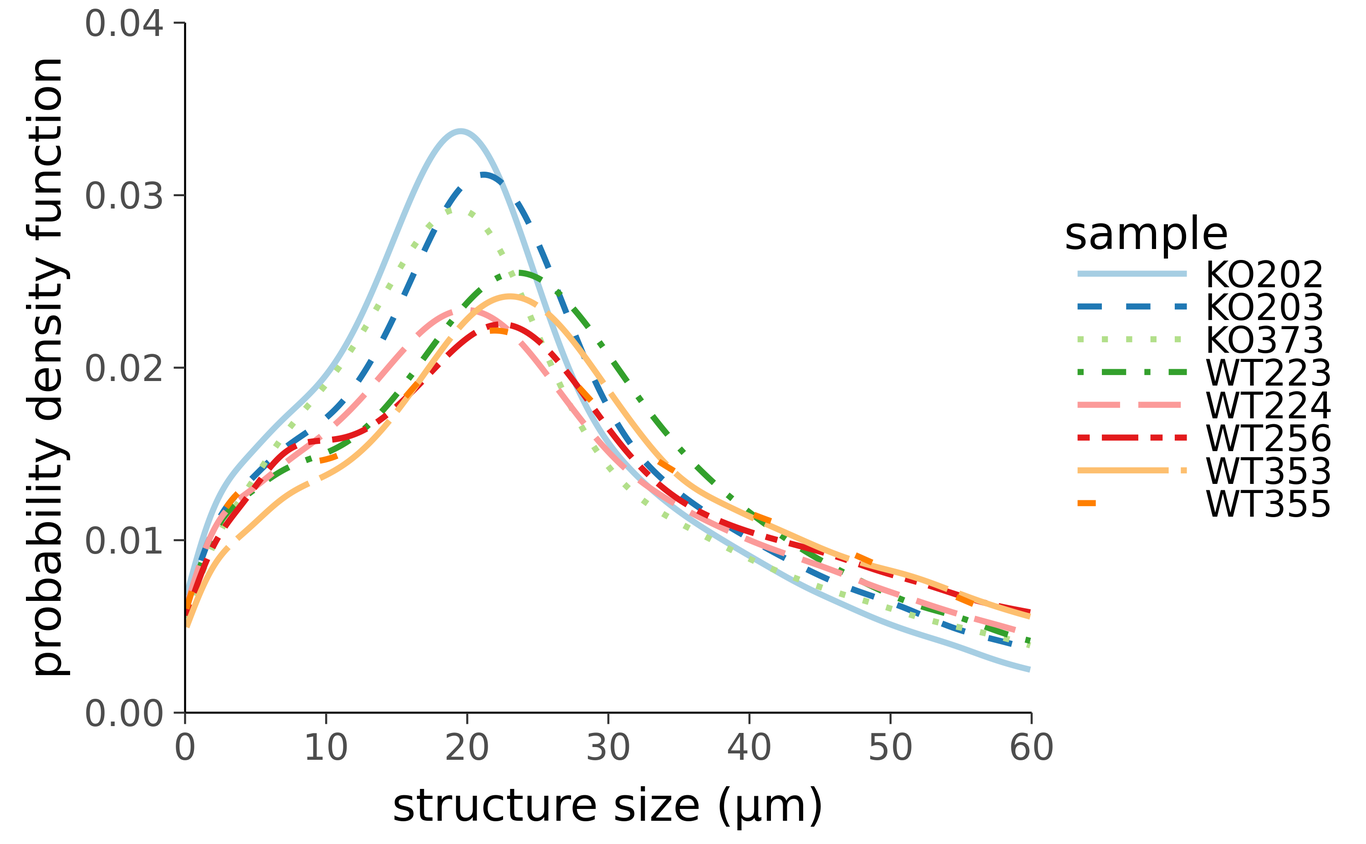
\includegraphics[width=0.70\columnwidth]{figures/size_pdf/size_pdf}
\caption{{Distribution of the diameters of the alveoli as determinedfrom
synchrotron tomography data for all samples.
{\label{243343}}%
}}
\end{center}
\end{figure}


\subsection*{Processing of the radiographic data}\label{sec:radioprocessing}
Radiographic data in the Talbot-Lau interferometer are recorded with the
following procedure. The interferometer is composed of three gratings,
labelled $G_0$, $G_1$ and $G_2$. The first grating $G_0$ creates an array of
individually coherent but mutually incoherent light sources from the
focal spot of the X-ray tube. The second grating $G_1$ generates an
interference pattern downstream by exploiting the self-imaging Talbot
effect. This interference pattern has the same periodicity of the grating
itself, 5.4 \selectlanguage{greek}μ\selectlanguage{english}m for the current experiment, and it is therefore too small to
be resolved by the detector. A third grating $G_2$ with the same period is
then moved in a direction perpendicular to the interference fringes over one
period in order to sample the intensity of the pattern at several positions.
This results in a so-called phase-stepping curve whose parameters change
when a sample is present in the beam: the average intensity is reduced
according to the absorption of the X-rays in the sample, while the reduction
in the amplitude of the curve is determined by microstructures.

A sinusoidal fit is performed with Fourier component analysis, where the
reference curve for each pixel is:

\begin{equation}
    c_f(x) = a_{0,f} + a_{1,f} \sin(x + \theta_{f}),
    \label{eqn:flat}
\end{equation}

the parameters are changed when a sample is in the beam:

\begin{equation}
    c_s(x) = a_{0,s} + a_{1,s} \sin(x + \theta_{s}).
    \label{eqn:sample}
\end{equation}

For each pixel, the transmission image $A$ and the
dark-field image $B$ are calculated (see fig.~\ref{590406}). Both of these
quantities are known to follow the Beer-Lambert law, with an exponential
decay related to the thickness $t$ of the sample: $A = \exp(-\mu_A t)$, $B =
\exp(-\mu_B t)$. Since the lung samples are irregular in shape, it is
beneficial to examine the ratio of the logarithms $R$ in
order to remove the local dependence on the thickness of the sample in the
radiography:

\begin{align*}
    A &= \dfrac{a_{0,s}}{a_{0,f}}\\
    B &= \dfrac{a_{1,s}}{a_{1,f}}\dfrac{a_{0,f}}{a_{0,s}}\\
    R &= \dfrac{\log(B)}{\log(A)}.
    \label{eqn:definitions}
\end{align*}\selectlanguage{english}
\begin{figure}[h!]
\begin{center}
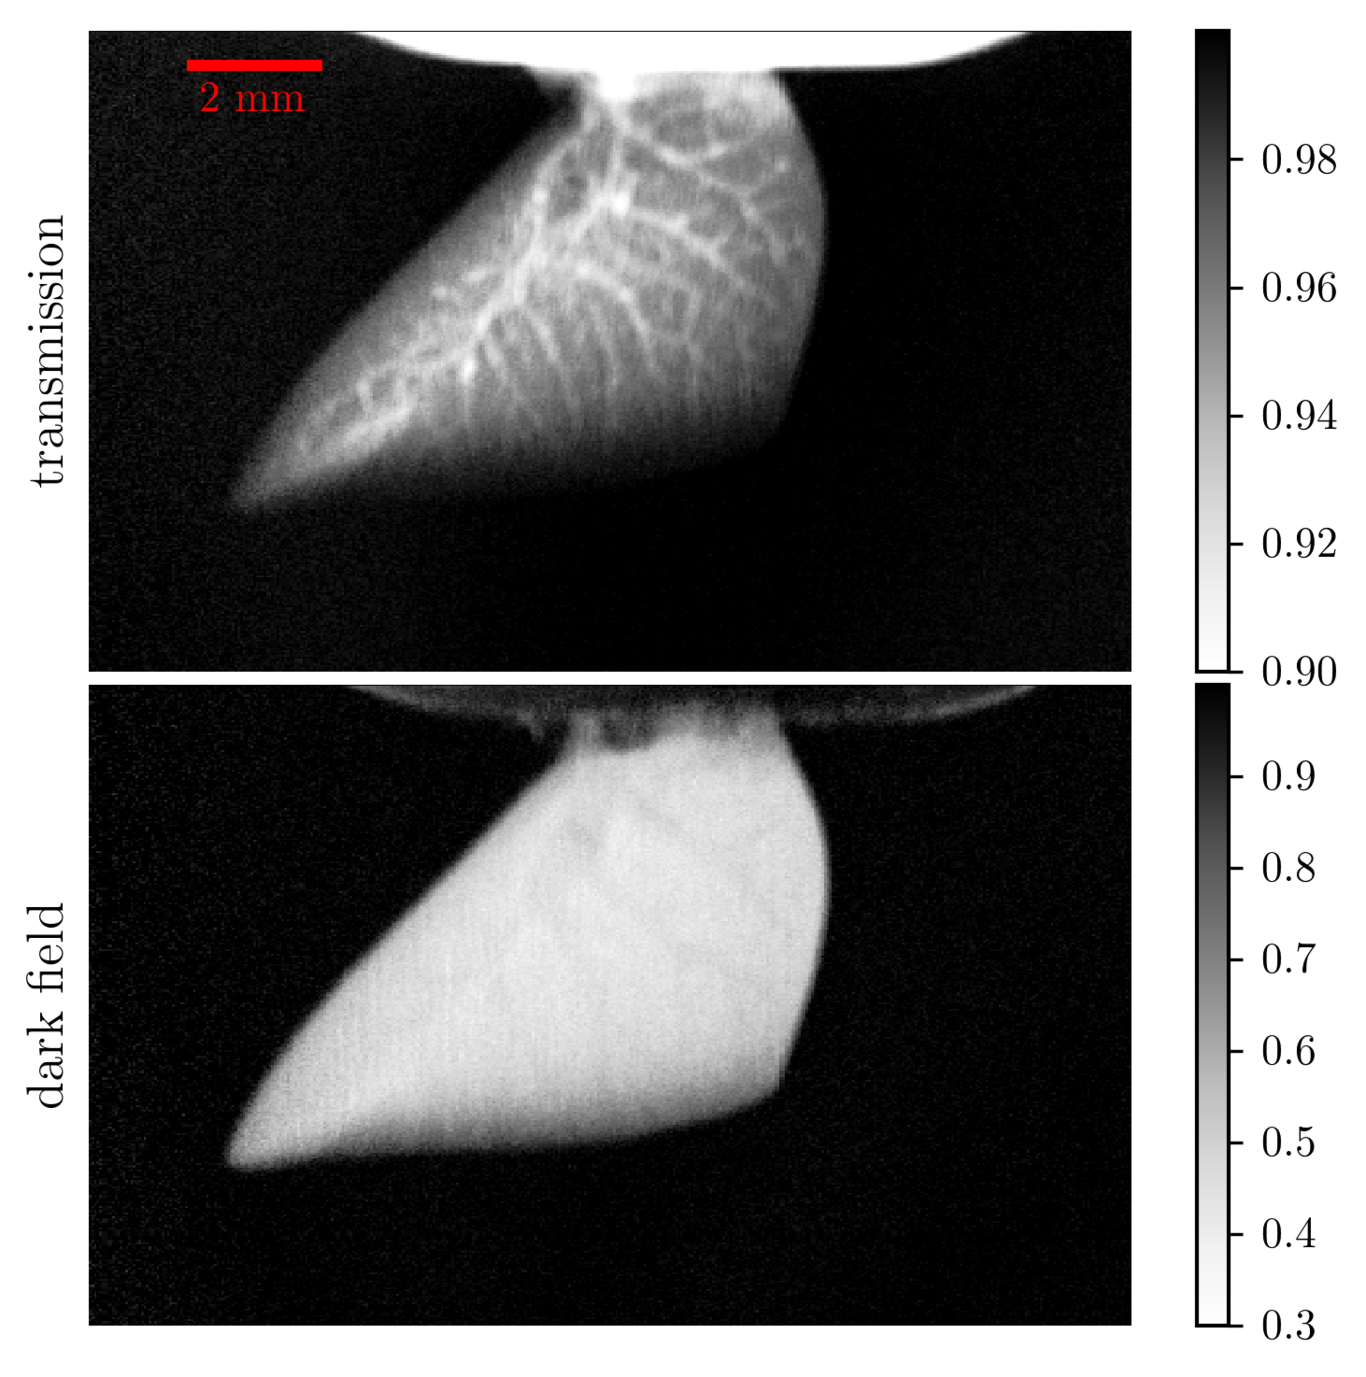
\includegraphics[width=0.70\columnwidth]{figures/KO373_LL_smoke/WT256_LL_smoke}
\caption{{Example of an ex vivo lung interferometric radiography on a laboratory
source. Sample WT256.
{\label{590406}}%
}}
\end{center}
\end{figure}

\section{Acknowledgements}
Part of this work has been funded by the ERC-2012-STG 310005-PhaseX grant.
The authors also thank Spyridon Gkoumas, Dectris Ltd., for the assistance
with the detector prototype and \dots, University of Bern, for the technical support in the
preparation of the samples.

\section{Author contributions}
M.A. and G.L. carried out the tomography scans. M.A. designed, realized and
operated the laboratory setup. M.A. and G.L. developed the theoretical
framework and performed the computations. T.C. prepared the lung samples
under the supervision of C.B. and J.S. M.S. supervised the findings of this
work. M.A., G.L. and J.S contributed to the final manuscript.

\selectlanguage{english}
\clearpage
\bibliographystyle{naturemag}
\bibliography{bibliography/biblio.bib}

\end{document}

